A fim de avaliar os resultados e a eficiência das heurísticas implementadas, criamos um processo para geração de instâncias do problema. Para criar um par de string balanceadas, escolhe-se: o número de rótulos replicados $r$ (ocorrência maior que 1), o número de singletons $s$ e o tamanho das strings $n$, sendo que $n \ge 2 \cdot r + s$. Uma string de inteiros é construída concatenando: duas cópias de cada inteiro em $[1, r]$, uma cópia de cada inteiro em $[r + 1, r + s]$ e $n - 2 \cdot r + s$ inteiros escolhidos aleatoriamente em $[1, r]$. Para obter o par de strings de entrada para o MCSP, duas permutações totalmente aleatórias da string formada são utilizadas.

Analisaremos na \Cref{sec:resultados-tempo} o tempo de execução dos algoritmos nos diferentes cenários, visando demonstrar as situações que favorecem algumas das heurísticas. Em seguida, na \Cref{sec:resultados-tamanho}, discutiremos o tamanho das partições resultantes para avaliar de fato cada um dos algoritmos. Para todos os testes realizados, exceto quando explicitado, fora utilizadas pelo menos 3000 diferentes instâncias do problema.

\subsection{Tempo de execução} \label{sec:resultados-tempo}

    O tempo de execução de cada um dos algoritmos é bem diferente, como pode-se observar na \Cref{tab:bench-tempo}. Enquanto o tempo para aplicar as heurísticas de combinação é da ordem de $\unit{\micro\second}$ e para a gulosa da ordem de $\unit{\milli\second}$, o PSO pode demorar vários segundos para ter sua execução finalizada, dependendo de seus parâmetros e das instâncias.

    É válido ressaltar também a diferença entre a variação do tempo de execução das heurísticas com os parâmetros de geração das strings. Enquanto o fator principal pelo aumento do tempo para os outros algoritmos é o tamanho das strings de entrada, o PSO é substancialmente mais rápido para instâncias com maior número de rótulos e, consequentemente, menor ocorrência média de seus rótulos. Essa dependência será mais explorada na \Cref{sec:tempo-pso}.

    \begin{table}[htb]
        \centering
        \begin{tabular}{ccc|cccc}
            \toprule
            $n$ & $r$ & $s$ & Combinação [$\unit{\micro\second}$] & Combinação-S [$\unit{\micro\second}$] & Gulosa [$\unit{\milli\second}$] & PSO [$\unit{\second}$] \\
            \midrule
            60 &  5 &  5 & 165 & 594  & 4.75 & 17.5 \\
            60 & 15 & 10 & 211 & 563  & 8.91 & 1.21 \\
            80 & 10 & 15 & 331 & 1140 & 17.4 & 5.79 \\
            80 & 20 & 30 & 401 & 1200 & 23.9 & 0.55 \\
            \bottomrule
        \end{tabular}
        \caption{Comparação de tempo de execução das diferentes heurísticas, relacionando cada conjunto de parâmetros de geração de strings ($n$, $r$ e $s$) ao tempo gasto por cada um dos algoritmos. Os valores de tempo foram obtidos através da média de execuções em diferentes instâncias, com a análise estatística realizada através da biblioteca \textit{Criterion} \cite{noauthor_criterion_nodate}. O PSO foi executado com $k_e = 0.5$, $k_i = 0.1$, $k_g = 0.1$, $D = (1, 3, 3, 3)$, 200 partículas e 100 iterações.}
        \label{tab:bench-tempo}
    \end{table}

    \subsubsection{Particle Swarm Optimization} \label{sec:tempo-pso}

        Analisando de forma mais detalhada o tempo de execução do PSO, espera-se que este dependa linearmente do número de arestas da representação por grafo da entrada do problema, já que praticamente todas as operações são feitas sobre vetores desse tamanho. De fato, a \Cref{fig:tempo-pso-vs-arestas} deixa clara essa dependência.

        O número de arestas do grafo, por sua vez, claramente tende a crescer com o tamanho das strings, mas ele está vinculado ainda mais à ocorrência dos caracteres: quanto maior a ocorrência dos caracteres de um bloco, maior tende a ser o número de blocos iguais a ele na outra string de entrada, formando assim mais arestas. A \Cref{fig:tempo-pso-arestas-vs-occ} mostra essa relação utilizando a ocorrência máxima das strings. Isso indica que o PSO é eficiente para casos em que os caracteres são replicados um número pequeno de vezes.

        \begin{figure}[htb]
            \centering
            \begin{subfigure}[b]{0.48\textwidth}
                \centering
                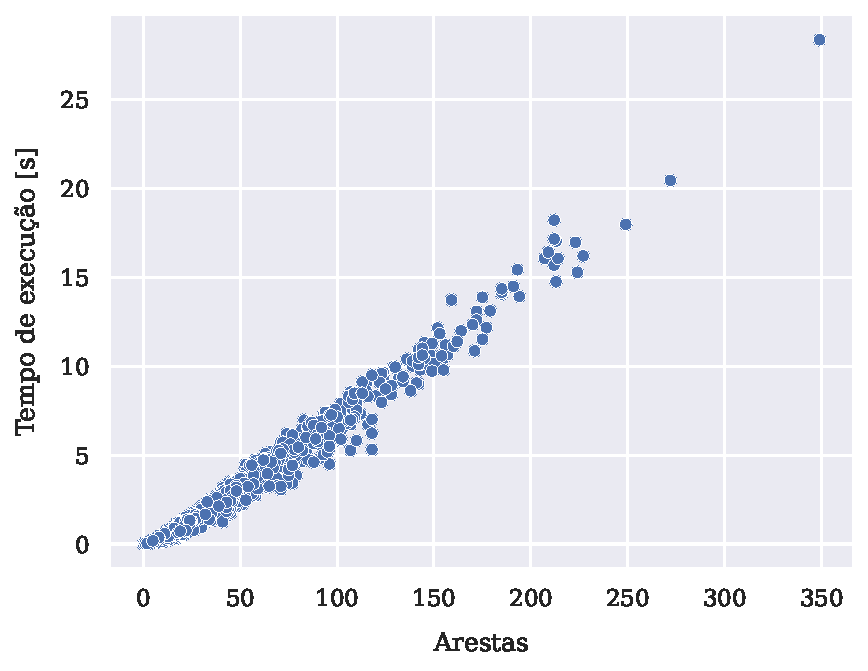
\includegraphics[width=\textwidth]{images/tempo-vs-arestas.pdf}
                \caption{Tempo de execução do PSO em função do número de arestas do grafo.}
                \label{fig:tempo-pso-vs-arestas}
            \end{subfigure} \hfill
            \begin{subfigure}[b]{0.48\textwidth}
                \centering
                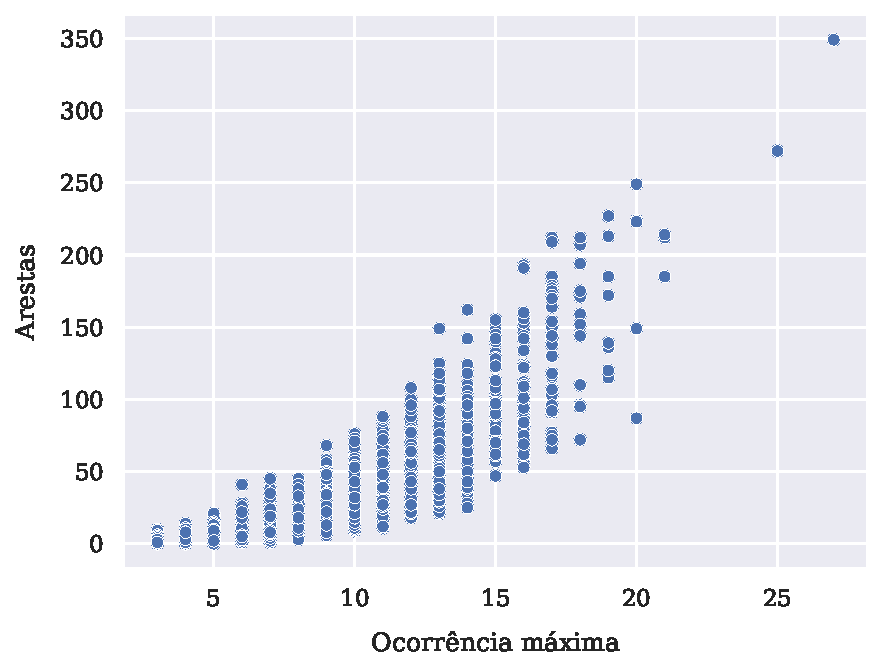
\includegraphics[width=\textwidth]{images/arestas-vs-occ.pdf}
                \caption{Número de arestas do grafo em função da ocorrência máxima das strings.}
                \label{fig:tempo-pso-arestas-vs-occ}
            \end{subfigure}
            \caption{Análise do tempo de execução do PSO. Note que o tempo depende linearmente do número de arestas da representação por grafo da instância de entrada, como esperado. Além disso, a grandeza que melhor permite prever o tempo de execução do algoritmo é a ocorrência máxima dos caracteres da string. As strings foram geradas usando $5 \leq r \leq 10$, $5 \leq s \leq 30$, $n \leq 80$. O PSO foi executado utilizando $k_e = 2$, $k_i = 0.02$, $k_g = 0.02$, $D = (3, 1, 1, 1)$, 10 partículas e 1000 iterações.}
            \label{fig:tempo-pso}
        \end{figure}

\subsection{Tamanho das partições} \label{sec:resultados-tamanho}

    Para avaliar o resultado da aplicação das heurísticas de forma independente do tamanho da string, definimos uma forma de pontuação, de forma que uma partição comum com apenas blocos unitários tem pontuação 0 e uma partição comum com apenas um bloco recebe pontuação 1. Note que raramente a solução ótima do MCSP recebe pontuação 1: isso ocorre apenas se as strings forem iguais.

    \begin{definition}[Pontuação]
        A pontuação de uma partição comum $\left(\part{P}, \part{Q}\right)$ de duas strings $A$ e $B$ é um valor em $[0, 1]$ que indica quão pequena $\left(\part{P}, \part{Q}\right)$ é em relação ao tamanho de $A$ e $B$. O valor da pontuação é dado por \[
            S \left(\part{P}, \part{Q}\right) = \frac{\abs{A} - \abs{\left(\part{P}, \part{Q}\right)}}{\abs{A} - 1}
        \]
    \end{definition}

    A \Cref{fig:comparacao-pontuacao} mostra a pontuação média das heurísticas para diferentes parâmetros de geração de strings. Em ambos os casos, o PSO conseguiu melhorar ligeiramente o resultado obtido pelos outros algoritmos (já que utiliza os outros resultados como posições iniciais). Uma análise mais específica da diferença obtida entre o PSO e as outras heurísticas pode ser vista na \Cref{fig:pso-diff}.

    \begin{figure}[htb]
        \centering
        \begin{subfigure}[b]{\textwidth}
            \centering
            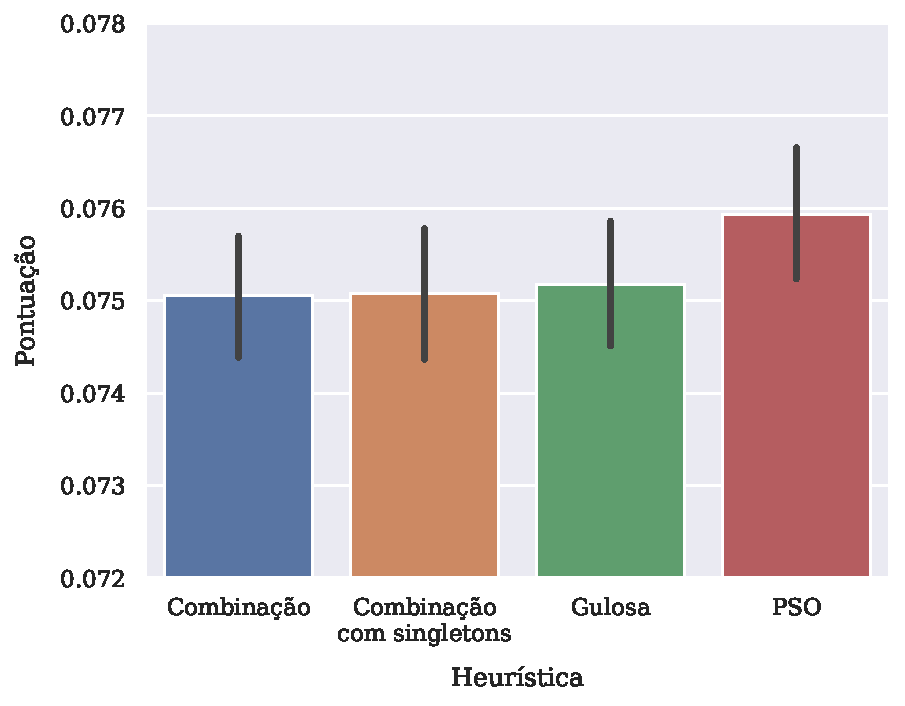
\includegraphics[width=0.5\textwidth]{images/r50-s-5-10-n220-ke0.5-ki0.1-kg0.1-dist1-3-3-3-iter100-part200.pdf}
            \caption{Strings geradas com $r = 50$, $5 \leq s \leq 10$ e $n \leq 220$.}
            \vspace{12pt}
        \end{subfigure}
        \begin{subfigure}[b]{\textwidth}
            \centering
            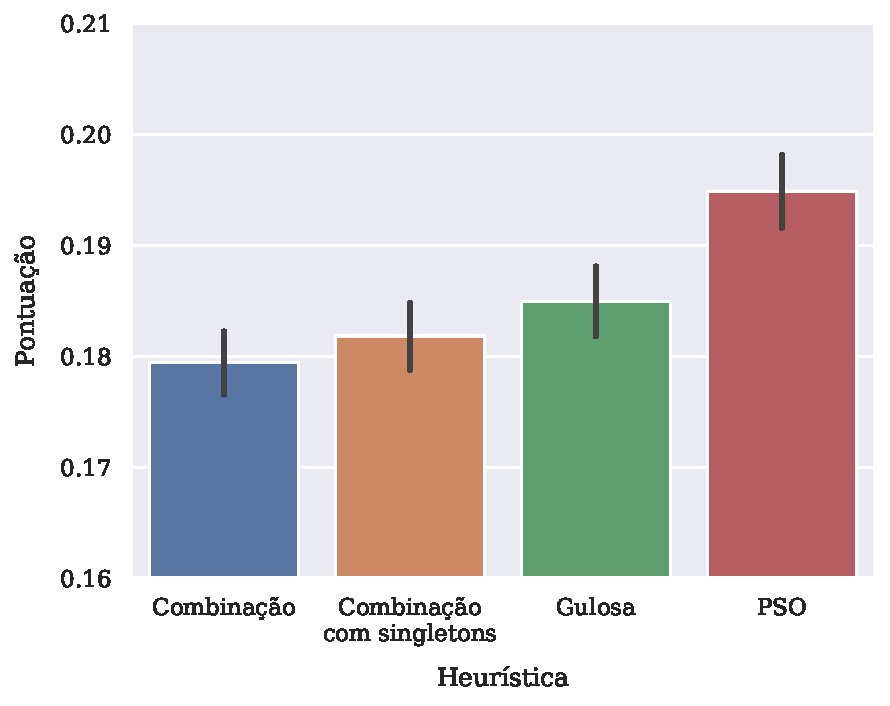
\includegraphics[width=0.5\textwidth]{images/r-5-10-s-5-30-n80-ke0.5-ki0.1-kg0.1-dist1-3-3-3-iter100-part200.pdf}
            \caption{Strings geradas com $5 \leq r \leq 10$, $5 \leq s \leq 30$ e $n \leq 80$.}
            \vspace{12pt}
        \end{subfigure}
        \caption{Comparação da pontuação média das heurísticas com diversos conjuntos de parâmetros de geração de strings. Em ambos os casos, o PSO foi utilizado com $k_e = 0.5$, $k_i = 0.1$, $k_g = 0.1$, $D = (1, 3, 3, 3)$, 200 partículas e 100 iterações.}
        \label{fig:comparacao-pontuacao}
    \end{figure}

    \begin{figure}[htb]
        \centering
        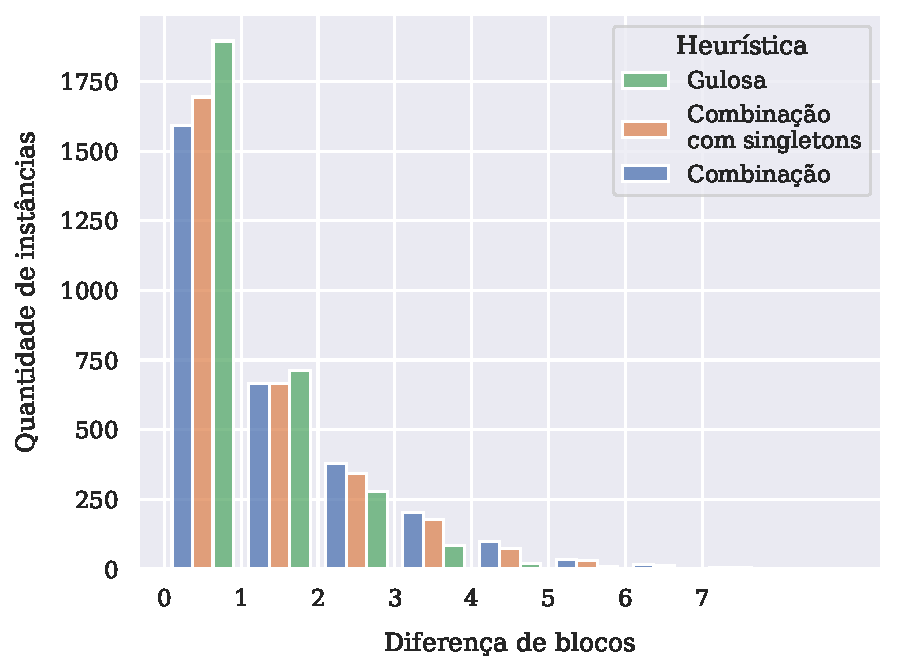
\includegraphics[width=0.5\textwidth]{images/pso-diff.pdf}
        \caption{Comparação entre o número de blocos resultantes da aplicação do PSO e das outras heurísticas. O gráfico mostra a distribuição da diferença entre o número de blocos obtidos pelo PSO e uma dada heurística na mesma instância do MCSP. Note que o resultado mais comum é o empate. Strings geradas com $5 \leq r \leq 10$, $5 \leq s \leq 30$ e $n \leq 80$. PSO executado com $k_e = 0.5$, $k_i = 0.1$, $k_g = 0.1$, $D = (1, 3, 3, 3)$, 200 partículas e 100 iterações.}
        \label{fig:pso-diff}
    \end{figure}

    \subsubsection{PSO com posições iniciais totalmente aleatórias}

        Até aqui analisamos o desempenho do PSO utilizando algumas das posições iniciais criadas a partir de resultados de outras heurísticas, de forma que seu resultado foi sempre no mínimo tão bom quanto ao da melhor heurística entre a gulosa e a combinação-S. A \Cref{fig:pso-puro} mostra uma comparação que inclui também o PSO com todas as posições iniciais sendo geradas de forma totalmente aleatória. Apesar de obter uma pontuação média ligeiramente menor que o algoritmo que inclui as outras formas de gerar posições iniciais, essa variação mais simples também foi capaz de obter melhores pontuações que as heurísticas gulosa e combinação-S, o que demonstra a eficácia do algoritmo, mesmo quando utilizando ``por si só''.

        \begin{figure}[htb]
            \centering
            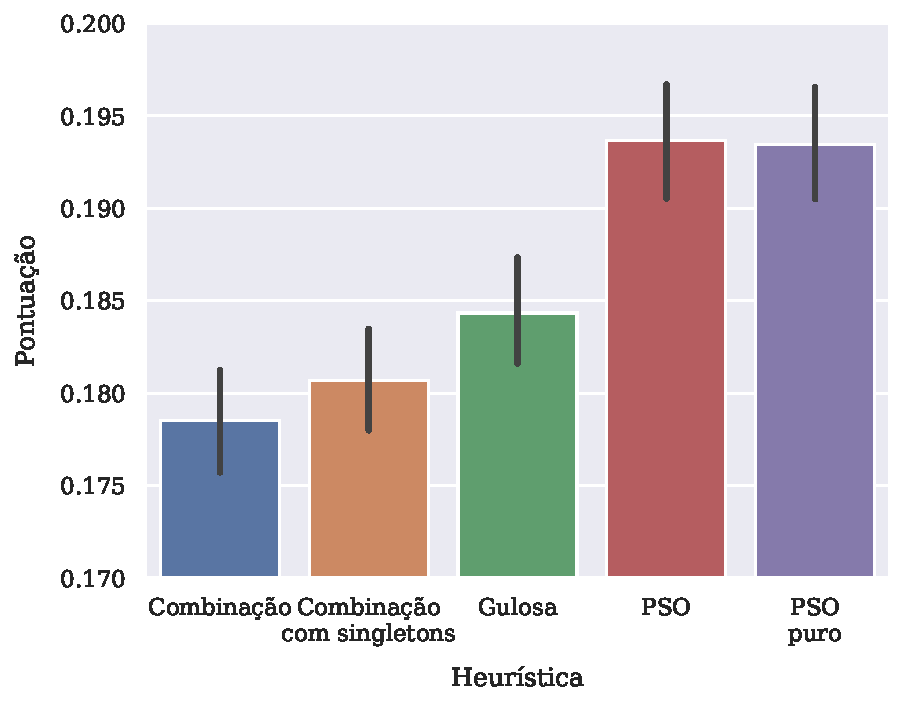
\includegraphics[width=0.5\textwidth]{images/pso-puro.pdf}
            \caption{Comparação entre a pontuação média das heurísticas, incluindo o PSO com posições inicias totalmente aleatórias. Apesar de haver uma ligeira diferença da pontuação média do PSO utilizando posições iniciais das outras heurísticas, o PSO com apenas posições iniciais aleatórias apresentou pontuação maior que as outras heurísticas. Strings geradas com $5 \leq r \leq 10$, $5 \leq s \leq 30$ e $n \leq 80$. PSO executado com $k_e = 2$, $k_i = 0.1$, $k_g = 0.1$, 200 partículas, 100 iterações e, para as execuções incluindo posições iniciais obtidas de outras formas, $D = (1, 3, 3, 3)$.}
            \label{fig:pso-puro}
        \end{figure}

    \subsubsection{Outros algoritmos da literatura}

        Além de comparar as heurísticas implementadas entre si, executamos também outros algoritmos desenvolvidos para o MCSP. Em um primeiro momento, utilizamos outras implementações das heurísticas gulosa e combinação-S disponíveis \cite{siqueira_signed_2023}. Ao aplicar as nossas e as outras implementações às mesmas instâncias do problema, obtivemos resultados idênticos.

        Comparamos também, para um conjunto restrito de instâncias pequenas, os resultados obtidos por um algoritmo de parâmetro fixo (FPT), que é exato para o MCSP, i.e. que sempre retorna uma solução ótima. A \Cref{fig:fpt} mostra que nenhuma das heurísticas acha de forma consistente a solução ótima para o problema, mas têm pontuações próximas a isso. A precisão desse conjunto de resultados é reduzida devido às restrições de quantidade e tamanho das instâncias, causadas pelo longo tempo necessário para executar o FPT. Ainda assim, é possível observar a tendência para cada um dos algoritmos.

        \begin{figure}[htb]
            \centering
            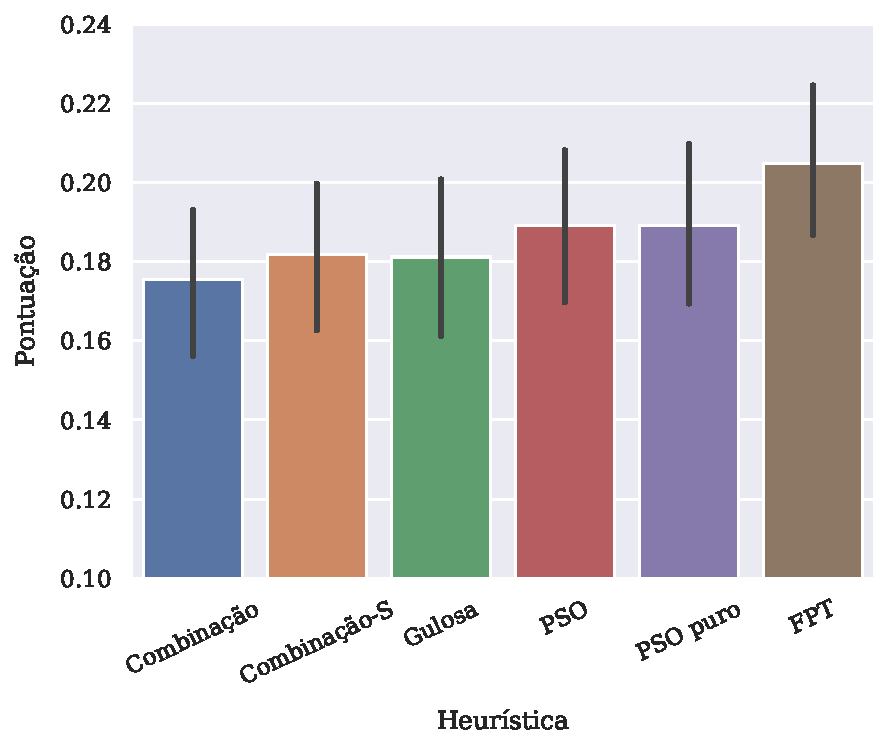
\includegraphics[width=0.5\textwidth]{images/fpt.pdf}
            \caption{Comparação entre a pontuação média dos algoritmos, incluindo o FPT. Os dados incluem apenas 72 instâncias, com strings geradas utilizando $5 \leq r \leq 10$, $2 \leq s \leq 30$ e $19 \leq n \leq 36$. PSO executado com $k_e = 2$, $k_i = 0.1$, $k_g = 0.1$, 200 partículas, 100 iterações e, para as execuções incluindo posições iniciais obtidas de outras formas, $D = (1, 3, 3, 3)$.}
            \label{fig:fpt}
        \end{figure}
